\begin{figure}[h!]
    \centering
    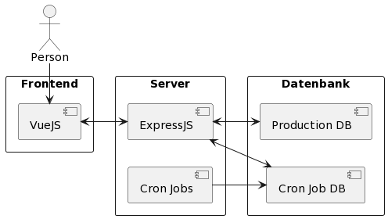
\includegraphics[width=1\textwidth]{pics/diplomarbeit-architektur.png}
    \caption{Systemarchitektur}
    \label{fig:mesh1}
\end{figure}

In dieser Grafik ist die Systemarchitektur des neuen Planfred Kundenmanagement Tools zu sehen. Der Benutzer:in kommuniziert dabei mit dem Frontend, welches auf einem VueJS Projekt basiert. Diese Anwendung schickt dann Anfragen an den Server, beziehungsweise bekommt Daten vom Server. Dieser basiert auf ExpressJS und bezieht Daten aus zwei verschiedenen Datenbanken:

\begin{itemize}
    \item \textbf{Production Datenbank}
        \newline
        Dabei handelt es sich um die Datenbank, welche auch bei dem eigentlichen Produkt Planfred zur Verwendung kommt. Das heißt, dass darauf alle Live-Daten gespeichert sind. Diese sind relevante Daten, wobei für uns die Informationen über die Kunden:innen und die dementsprechenden Projekte am wichtigsten waren.
        Hierbei ist es auch wichtig zu erwähnen, dass es sich dabei um eine MongoDB Datenbank handelt und damit NoSQL verwendet wird.
        NoSQL-Datenbanken sind nicht-relationale Datenbanken, die flexibel skalierbar sind und verschiedene Datenformate unterstützen, um Daten effizient abzurufen und Joins zwischen Tabellen zu vermeiden.
        \cite{no_sql}
    \item \textbf{Cron Job Datenbank}
        \newline
        Es handelt sich dabei um eine zusätzliche Datenbank, welche Daten aus den Cron Jobs abspeichert. Diese Daten haben auf der Production-DB nichts verloren, da sie nur vom Kundenmanagement Tool verwendet werden und dadurch bewusst davon abgetrennt wurden.
        Es handelt sich hierbei ebenfalls um eine MongoDB Datenbank.
\end{itemize}

Wie gerade erwähnt wurde, werden Cron Jobs verwendet. Diese sind dafür da, um durch aufwändige Abfragen keine Performance zu verlieren. Dabei werden diese problematischen Abfragen nur einmal am Tag, extern vom Rest der Technologien, auf einen eigenen Server abgerufen und die Ergebnisse auf der Cron Job Datenbank gespeichert. Dadurch hat man im Kundenmanagement Tool zwar nicht immer die aktuellsten Daten von einigen Bereichen, dies spart aber wichtige Zeit und stellt gleichzeitig kein Problem dar.
